\documentclass[a4paper, 12pt]{article}

\usepackage{hyperref}
\usepackage{fullpage}
\usepackage[top=0.5in, bottom=1.5in, left=0.5in, right=0.5in, footskip=4em]{geometry}
\usepackage{amsmath}
\usepackage{fancyhdr}
\usepackage[usenames,dvipsnames]{xcolor}
\usepackage{pgfornament}

\usepackage[shortlabels]{enumitem}
\usepackage{xspace}
\usepackage{lastpage}
\usepackage{multicol}
\usepackage{blindtext}
\usepackage{titling}
\usepackage{standalone}
\usepackage{amsfonts}
\usepackage[framemethod=TikZ]{mdframed}
\usetikzlibrary{calc}
\usepackage{lineno}
\usepackage{amsthm}
\usepackage{amssymb}
\usepackage{mathtools}
\usepackage{datetime}
\usepackage[most]{tcolorbox}
\usepackage{cancel}
\usepackage{ulem}
\usetikzlibrary{tikzmark, trees, backgrounds}
\usepackage{pgfplots}
\linenumbers
\usepackage{tikz-qtree}

%BEGIN_FOLD Commands
\usepackage{amssymb}% http://ctan.org/pkg/amssymb
\usepackage{pifont}% http://ctan.org/pkg/pifont
\newcommand{\cmark}{\ding{51}}%
\newcommand{\xmark}{\ding{55}}%
\newcommand{\half}{\ensuremath{\frac{1}{2}}}
\newcommand{\epv}[1]{\ensuremath{\left< #1 \right>}\xspace}
\newcommand{\variance}{\ensuremath{\text{Var}}}
\newcommand{\eout}{\ensuremath{E_\text{out}}\xspace}
\newcommand{\ein}{\ensuremath{E_\text{in}}\xspace}
\newcommand{\cx}{\ensuremath{\mathcal{X}}\xspace}
\newcommand{\cz}{\ensuremath{\mathcal{Z}}\xspace}
\newcommand{\real}{\mathbb{R}}
\DeclareSymbolFont{extraup}{U}{zavm}{m}{n}
\DeclareMathSymbol{\varheart}{\mathalpha}{extraup}{86}
\DeclareMathSymbol{\vardiamond}{\mathalpha}{extraup}{87}
\renewcommand{\heartsuit}{\textcolor{red}{\varheart}}
\renewcommand{\diamondsuit}{\textcolor{red}{\vardiamond}}
\newcommand{\definition}{\vspace{1em}\noindent\textbf{Def:} }
\newcommand{\theorem}{\vspace{1em}\noindent\textbf{Theorem:} }
\newcommand{\collorary}{\vspace{1em}\noindent\textbf{Theorem:} }
\newcommand{\example}{\vspace{1em}\noindent\textbf{Example:} }
\newcommand{\solution}{\newline\noindent\textbf{Solution:} }
\newcommand{\predicate}{\vspace{0.25em}\noindent\textbf{Inductive Predicate:} }
\newcommand{\inductivestep}{\vspace{0.25em}\noindent\textbf{Inductive Step:} }
\renewcommand{\proof}{\vspace{0.5em}\noindent\textbf{Proof:} }
\newcommand{\lemma}{\vspace{1em}\noindent\textbf{Lemma:} }
\newcommand{\hint}{\textbf{Hint:} }
\newcommand{\basecase}{\vspace{0.25em}\noindent\textbf{Base Case:} }
\newcommand{\inductivehypothesis}{\vspace{0.25em}\noindent\textbf{Inductive Hypothesis:} }
\renewcommand{\collorary}{\vspace{1em}\noindent\textbf{Collorary:} }
\newcommand{\qedd}{\qed\newline}
\newcommand{\kwd}[1]{\textcolor{blue}{\textbf{\underline{#1}}}}
\newcommand\ColorBox[2][]{%
	\stepcounter{mybox}%
	\node[draw=red!70!black,fill=red!20,align=left,#1] (box\themybox) {#2};
}
\newcommand{\expl}[2]{%
	\underset{\substack{\uparrow\\\mathrlap{\text{\hspace{-1em}#2}}}}{#1}}
\newcommand{\uexpl}[2]{%
	\overset{\substack{\mathrlap{\text{\hspace{-1em}#2}}\\\downarrow}}{#1}}
\newcommand{\st}{\text{ such that }}
\newcommand{\R}{\textcolor{red}{R}}
\newcommand{\sumn}{\sum^n_{i=0}}
\newcommand{\sumxn}{\sum^n_{x=0}}
\newcommand{\red}[1]{\textcolor{red}{#1}}
\newcommand{\blue}[1]{\textcolor{blue}{#1}}
%\newcommand{\qed}{\ensuremath{\blacksquare}}
%END_FOLD
\newcommand{\sidenote}[1]{\textcolor{gray}{#1}}
\let\Pr\relax
\DeclareMathOperator{\Pr}{Pr}
\DeclareMathOperator{\E}{\mathbb{E}}
\DeclareMathOperator{\Cov}{Cov}
%BEGIN_FOLD miscellaneious default
\makeatletter
% Make a copy of macros responsible for entering display math mode
\let\start@align@nopar\start@align
\let\start@gather@nopar\start@gather
\let\start@multline@nopar\start@multline
% Add the "empty line" command to the macros
\long\def\start@align{\par\start@align@nopar}
\long\def\start@gather{\par\start@gather@nopar}
\long\def\start@multline{\par\start@multline@nopar}
\makeatother
\setlength{\columnsep}{1cm}
%opening
\setlength{\abovedisplayskip}{-\baselineskip}%
\setlength{\abovedisplayshortskip}{\abovedisplayskip}%

\pagestyle{fancy}
\renewcommand{\headrulewidth}{0pt}
\lfoot{\small{\course}: Week \weekno}
\rfoot{\small{\thetitle}}
\rhead{}
\cfoot{\pgfornament[height=1em, ydelta=-0.4em]{17} \thepage of \pageref{LastPage}  \pgfornament[height=1em, ydelta=-0.4em]{18}}

\DeclareMathOperator{\sign}{sign}
\DeclareMathOperator{\Var}{Var}
\newcommand{\vect}[1]{\ensuremath{\mathbf{#1}}\xspace}

\tikzstyle{every picture}+=[remember picture]
\newcommand{\bwgrid}[1]{
	\def \aaa #1
	
	\foreach \y in {0,1,2} {
		\foreach \x in {0,1,2} {
			\pgfmathsetmacro{\clr}{\aaa[\x][\y]}
			%\message{aaa \clr}
			\definecolor{MyColor}{rgb}{\clr,\clr,\clr}
			\path[fill=MyColor] (\x,\y) rectangle ++(1,1); 
		}
	}
	\draw[step=1cm,very thin] (0,0) grid (3,3);	
}

\setenumerate{label=\alph*.)}
\definecolor{db}{RGB}{100,65,23}

%END_FOLD

\newcommand{\course}{Discrete Math}
\title{Random Vairable and Expected Value}
\newcommand{\weekno}{9}

\begin{document}
\begin{center}
	\textcolor{orange}{\textsc{\course}}\\
	\huge\textbf{\textsc{\thetitle}}\\
	\small\textcolor{gray}{Last updated:\, \today \, \currenttime}\\
	\pgfornament[width=0.7\textwidth, color=white!30!black]{88}
\end{center}


\begin{multicols}{2}
	
\section*{Random Variable}
Let us consider tossing 3 coins. We can talk about the number of head of each outcome and ask about what is the probability of each event.
\begin{itemize}
	\item 0 Head = $\{TTT\}$
	\item 1 Head = $\{HTT, THT, TTH\}$
	\item 2 Heads = $\{HHT, HTH, THH\}$
	\item 3 Heads = $\{HHH\}$
\end{itemize}

This means that given an outcome we can find out the number of head. This is called a Random Variable. A number that depends on the outcome.

\definition Random Variable, $R$, is a function from sample space $S$ to a real number $R:S\to \real.$

\vspace{1em}
For example, if $R$ is the random variable for the number of head then $R(TTT)=0, R(HTT)=1, R(HHT)=2$ etc.

Another example would be a random variable $M$ which is defined as
\begin{equation*}
	M(\omega) = \begin{cases*}
		1 & \text{if all three coins match}\\
		0 & \text{otherwise}\\
	\end{cases*}
\end{equation*}
Then, this means $M(TTT)=1, M(HHH)=1, M(HHT)=0$ etc.

We can then talk about the probability that a random variable attain certain value. Natuarally, we want
\[
	\Pr(R = 2) = \Pr(HHT) + \Pr(HTH) + \Pr(THH)
\]
This leads us the the definition
\[
	\Pr(R=x) \equiv \sum_{\omega \text{ s.t.} R(\omega) = x } \Pr(\omega)
\]
just the sum of the probability of the outcome that gives the desired outcome.

We can also talk about the probability that the random vairable will attain the value in some range for example
\begin{align*}
	\Pr(R \ge 2) =& \Pr(HHT) + \Pr(HTH) + \Pr(THH)+ \\
	& \Pr(HHH)
\end{align*}

\subsection*{Conditional and Indepenent}

We can also do \emph{conditional} probability on the random variable.
\[
	Pr(R=2 | M = 0) = \frac{\Pr(R=2 \cap M=0)}{\Pr(M=0)}
\]

That means we can also define independent on the random variable

\definition Two random variables $R_1$ and $R_2$ are \emph{independent} iff $\forall x_1, x_2 \in \real$
\begin{gather*}
	\Pr(R_1=x_1 | R_2=x_2) = \Pr(R_1=x_1) \\
	\text{or} \\
	\Pr(R_2 = x_2) = 0
\end{gather*}
This means that knowing the value of one of the random variable tell you nothing about the value of the other random variable.

Also, like independe of events we have an equivalent definition(you can prove this as an exercise) that

\definition Two random variables $R_1$ and $R_2$ are \emph{independent} iff $\forall x_1, x_2 \in \real$
\[
	\Pr(R_1=x_1 \cap R_2 = x_2) = \Pr(R_1=x_1) \times \Pr(R_2=x_2)
\]
This is a bit easier to use than the first definition.

\example Are $M$ and $R$ independent?

No.
\[
	\Pr(R=2 \land M=1) = 0 \ne \Pr(R=2) \times \Pr(M=1)
\]

\example Let us consider tossing two fair independent 6 sided dice.
\begin{itemize}
	\item Let $D_1$ be the random variable for the value of the first dice.
	\item Let $D_2$ be the random variable for the value of the second dice.
	\item Let $S=D_1+D_2$ this means that $S$ is a random variable for the sum of the two dice.
	\item Let $T$ be define as follow
	\[
		T = \begin{cases}
		1 & \text{if }S=7\\
		0 & \text{otherwise}
		\end{cases}
	\]
\end{itemize}
The first question is whether $S$ and $D_1$ are independent. This is not the case since
\[
	Pr(S=12 \land D_1 = 1) = 0 \ne \Pr(S=12)\Pr(D_1=1)
\]

Next question is whether $T$ and $D_1$ are independent. To check whether they are independent, you need to check all the possible combinations of the value for $T$ and $D_1$. This means we need to check for
\begin{align*}
	\Pr(T=1|D_1=1) = \frac{1}{6} = Pr(T=1) & \checkmark\\
	\Pr(T=1|D_1=2) = \frac{1}{6} = Pr(T=1) & \checkmark\\
	\Pr(T=1|D_1=3) = \frac{1}{6} = Pr(T=1) & \checkmark\\
	\Pr(T=1|D_1=4) = \frac{1}{6} = Pr(T=1) & \checkmark\\
	\Pr(T=1|D_1=5) = \frac{1}{6} = Pr(T=1) & \checkmark\\
	\Pr(T=1|D_1=6) = \frac{1}{6} = Pr(T=1) & \checkmark\\
	\Pr(T=0|D_1=1) = \frac{5}{6} = Pr(T=0) & \checkmark\\
	\Pr(T=0|D_1=2) = \frac{5}{6} = Pr(T=0) & \checkmark\\
	\Pr(T=0|D_1=3) = \frac{5}{6} = Pr(T=0) & \checkmark\\
	\Pr(T=0|D_1=4) = \frac{5}{6} = Pr(T=0) & \checkmark\\
	\Pr(T=0|D_1=5) = \frac{5}{6} = Pr(T=0) & \checkmark\\
	\Pr(T=0|D_1=6) = \frac{5}{6} = Pr(T=0) & \checkmark\\
\end{align*}
This means that $T$ and $D_1$ are independent.

\section*{Probability Distribution}

\definition Given a random variable $R$ the \emph{probability distribution function} (pdf) for $R$ is
\[
	f(x) = \Pr (R=x)
\]

\definition The cumulative distribution function $F$(cdf).
\[
	F(x) = \Pr(R\le x)
\]

\example Suppose that we toss an unfair coin(head with probability $p$ and tail with probability $(1-p)$). Let us define a random variable
\[
	R(\omega) = \begin{cases}
		1 & \text{if it is head}\\
		0 & \text{otherwise}
	\end{cases}
\]
The probability distribution function of $R$ is given by
\[
	f_R(x) \text{ such that } f_R(0) = 1-p, f_R(1)=p
\]
since the probability of $R$ being 0 is $1-p$ and the probability of $R$ being $1$ is $p$.

The cumulative distribution function of $R$ is given by
\[
	c_R(x) \text{ such that } c_R(0) = 1-p, c_R(1) = 1
\]

\example suppose we toss two unfair coins( $p$ for head and $1-p$ for tail). Let us define
\[
	R(\omega) = \text{Number of heads in }\omega
\]
then the probability distribution function for $R$ is given by
\begin{center}
	$f_R(\omega) $\\
	\text{ such that }\\
	$f_R(0) = (1-p)^2, f_R(1) = 2p(1-p), f_R(2) = p^2$
\end{center}

\example Let us consider a uniform random variable on $[1,n]$. This means the probability that the random variable taking any value in that range is equal. This means the probability distribution function is 
\[
	f(k) = \frac{1}{n}
\]
and the cdf is given by
\[
	C(k) = \frac{k}{n}
\]
Uniform random variable is a very important distribution let us do one more example

\section*{Envelope Game}
We have two envelopes. Each has the number from $[0,n]$ on it.
\begin{enumerate}
	\item First you pick one envelope and open it.
	\item Then, you decide whether to switch the envelope.
	\item If you end up with the envelope with greater number you win.
\end{enumerate}
The question is whether this game is 50\%-50\%. Can you beat 50-50 chance?

Consider the strategy where we set a random threshold($g$) from the set 
\[
	G = \{ \frac{1}{2}, 1 \frac{1}{2}, 2\frac{1}{2}, \ldots \}
\]
from a uniform distribution then if the number you pick is less than $g$ then you switch. Let us calculate the probability that you will win using this strategy.

Let the numbers on the two envelopes be $x$ and $y$. Without loss of generality let $y<x$. Then we start guessing the number $g$ from the set $G$. 
\end{multicols}

\begin{center}
	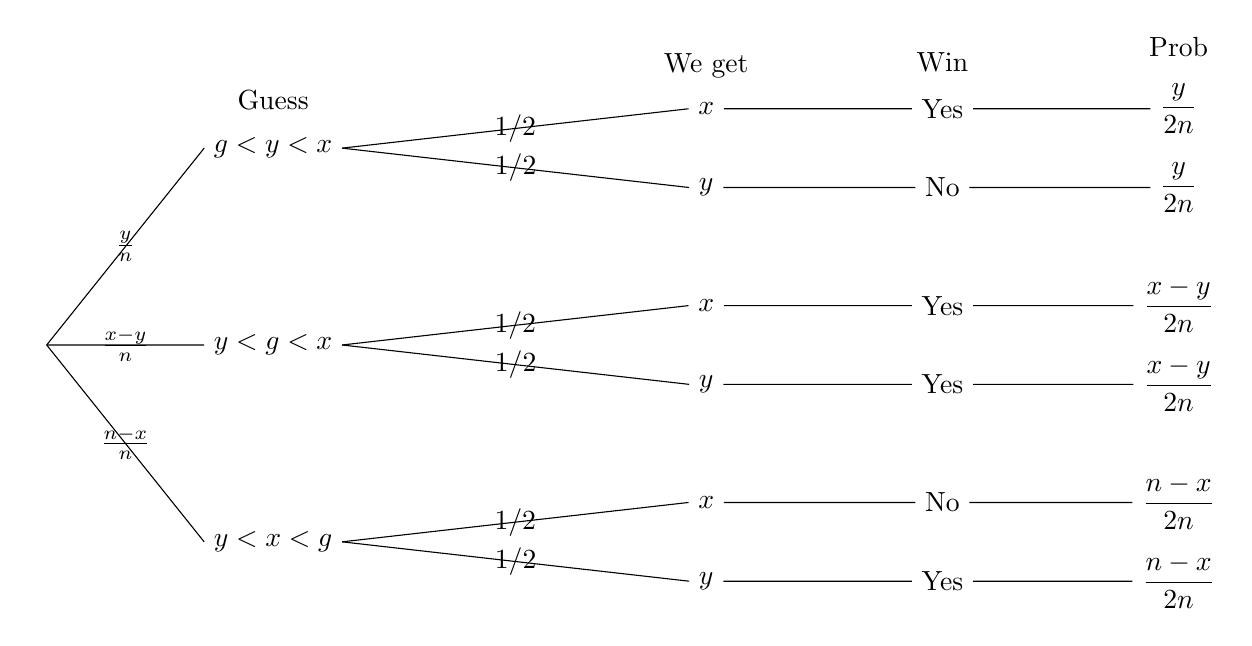
\begin{tikzpicture}[grow'=right,
	level 1/.style={sibling distance=2.5cm, level distance=3cm},
	level 2/.style={sibling distance=1cm, level distance=5.5cm},
	level 3/.style={level distance=3cm}]
	\node{}
	child{
		node(guess){$g<y<x$}
		child{
			node(x) {$x$}
			child {
				node(no) {Yes}
				child {node(prob){$\displaystyle \frac{y}{2n}$}}
			}
			edge from parent node{$1/2$}
		}
		child{
			node{$y$}
			child {
				node{No}
				child {node{$\displaystyle \frac{y}{2n}$}}	
			}
			edge from parent node{$1/2$}
		}
		edge from parent node{$\frac{y}{n}$}
	}
	child{
		node{$y<g<x$}
		child{ 
			node{$x$}
			child {
				node{Yes}
				child {node{$\displaystyle \frac{x-y}{2n}$}}	
			}
			edge from parent node{$1/2$} 
		}
		child{
			node{$y$}
			child {
				node{Yes}
				child {node{$\displaystyle \frac{x-y}{2n}$}}	
			}
			edge from parent node{$1/2$}
		}
		edge from parent node{$\frac{x-y}{n}$}
	}
	child{
		node{$y<x<g$}
		child{
			node{$x$} 
			child {
				node{No}
				child{ node{$\displaystyle \frac{n-x}{2n}$}}	
			}
			edge from parent node{$1/2$}
		}
		child{
			node{$y$} 
			child {
				node{Yes}
				child{ node{$\displaystyle \frac{n-x}{2n}$} }	
			}
			edge from parent node{$1/2$}
		}
		edge from parent node{$\frac{n-x}{n}$}
	};
	\node[yshift = 1em] at (no.north) {Win};
	\node[yshift = 1em] at (x.north) {We get};
	\node[yshift = 1em] at (guess.north) {Guess};
	\node[yshift = 1em] at (prob.north) {Prob};
\end{tikzpicture}
\end{center}
\begin{multicols}{2}
	So that means using a uniform guess $g$ has the probability of winning of
\begin{align*}
	P_{win} =& \frac{y}{2n} + \frac{x-y}{2n} + \frac{x-y}{2n} + \frac{n-x}{2n}\\
	&= \frac{n}{2n} + \frac{x-y}{2n}\\
	&= \frac{1}{2} + \frac{x-y}{2n}\\
	&> \frac{1}{2} &\text{ since $x>y$}
\end{align*}
That means uniform guess give you more than 50-50 change of winning.

\section*{Binomial Distribution}

Consider tossing $n$ unfair coins where the probability of getting head is $p$ and the probability of getting a tail is $1-p$.

If you toss the coin $n$ times then what is the probability of getting $k$ head?

Since for $k$ heads there are $\displaystyle {n \choose k}$ ways to do that and the probability of getting each of them is is $p^k(1-p)^{n-k}$. So that means that
\[
	f(k; n) = {n \choose k}p^k(1-p)^{n-k}
\]

This is actually one of the most important distribution of all. The assumption that give rises to the pdf is so simple. All you need is the same repeated experiment each with probability $p$.

\example Consider an LCD on your computer screen. Retina display has $2560\times1600$ which is about 4 million pixel. And there are three color so in total you have 12 million pixel.

Suppose you get an LED that is so good in production that only 1 in a 10 million will fail with in a year. If you calculate the probability that none of the LED in the 12 million pixel will fail in a year. You will find that only 30\% of the screen will pass the test. If you raise requirement to 1 pixel then it's $66\%$. Even if we allow two which is quite bad already, it is just $89\%$. So, you should feel very very lucky that your screen doesn't have a bad pixel.

%\section*{Poisson Distribution}
%
%A lot of time the number of our trail is large(sometimes it is unkowningly large) and the probability is small using the binomial distribution for the number of occurence give you the exact answer...

\section*{Expected Value}

\definition The expected value(mean) of a random variable $R$ over the probability space $S$ is given by
\[
	\E(R) = \sum_{\omega \in S}^{} R(\omega) \Pr(\omega)
\]

\example Consider rolling a fair 6-sided dice and let $R$ be the random variable fo the dice face.
\begin{align*}
	\E(R) =& 1\times\frac{1}{6} + 2 \times \frac{1}{6} + 3 \times\frac{1}{6}+\\
	&4\times\frac{1}{6} + 5 \times \frac{1}{6} + 6 \times\frac{1}{6}\\
	=& 3 \frac{1}{2} \leftarrow \text{not in any of $R(\omega)$}
\end{align*}

\definition The meandian of a random variable $R$ is $x\in R(\omega)$ such that
\[
	\Pr(R\le x) =\half
\]
and
\[
\Pr(R>x) =\half
\]

\example The median of $R$ defined above is $4$.
\end{multicols}
\section*{Flipping a Coin}

Consider the following coin toss game of 3 player.
\begin{itemize}
	\item At the beginning of the game each player bet 2 Baht on head or tail.
	\item So, we have the pot of 6 Baht.
	\item We then toss the coin. All those who pick the right side split the pot. Specifically, there there is one winner then the winner gets 6 Baht. If there are two winners then each get 3 Baht. If there is no winner of there are three winner then each get 2 Baht.
\end{itemize}

If all player bets at random then the expected value of gain is exactly 0. The tree show below is just the first half the other half is symmetric.
\[
	\E(\text{Gain}) = 2\times \frac{1}{16}(0+0+1-2+1-2+4-2) = 0
\]



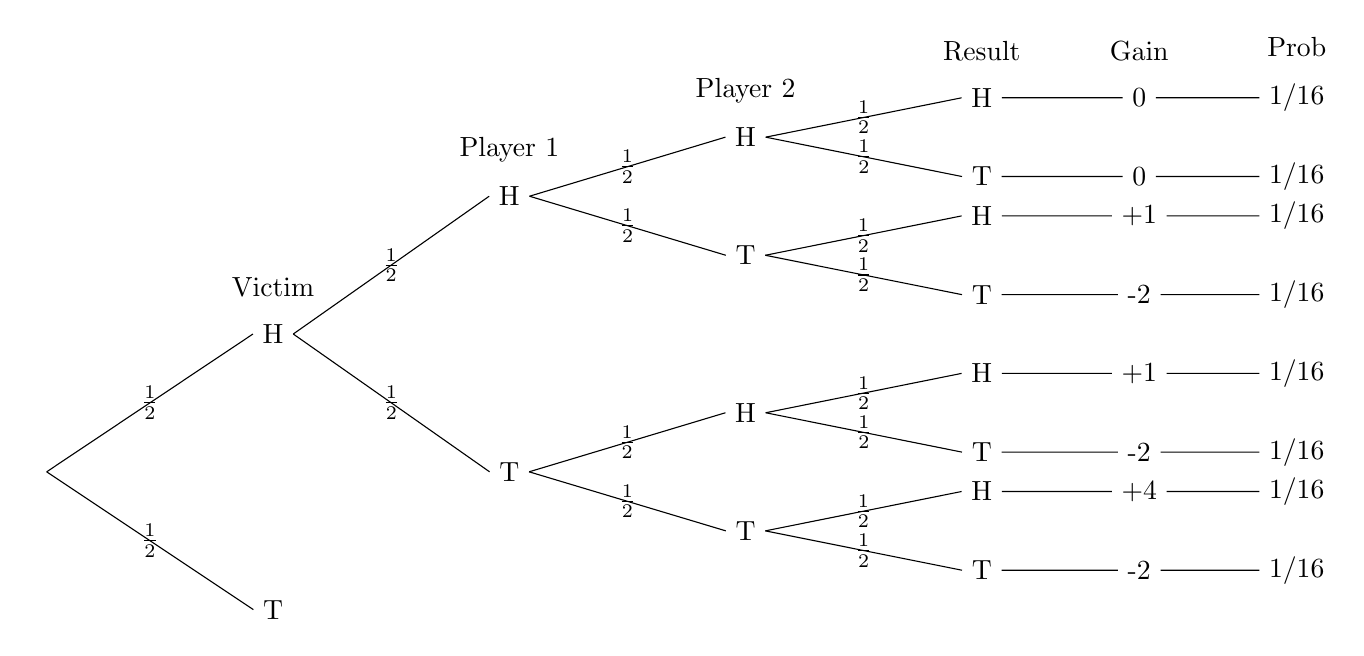
\begin{tikzpicture}[grow'=right,
	level 1/.style={sibling distance=3.5cm, level distance=3cm},
	level 2/.style={sibling distance=3.5cm, level distance=3cm},
	level 3/.style={sibling distance=1.5cm},
	level 4/.style={sibling distance=1cm},
	level 5/.style={level distance = 2cm}]
	\node {}
	child{
		node(victim){H}
		child{
			node(p1){H}
			child{
				node(p2) {H}
				child{
					node(actual) {H}
					child{
						node(gain) {0}
						child{
							node(prob) {1/16}
						}
					}
					edge from parent node {\half}
				}
				child{
					node {T}
					child{
						node {0}
						child{
							node {1/16}
						}
					}
					edge from parent node {\half}
				}
				edge from parent node {\half}
			}
			child{
				node {T}
				child{
					node {H}
					child{
						node {+1}
						child{
							node {1/16}
						}
					}
					edge from parent node {\half}
				}
				child{
					node {T}
					child{
						node {-2}
						child{
							node {1/16}
						}
					}
					edge from parent node {\half}
				}
				edge from parent node {\half}
			}
			edge from parent node {\half}
		}
		child{
			node{T}
			child{
				node {H}
				child{
					node {H}
					child{
						node {+1}
						child{
							node {1/16}
						}
					}
					edge from parent node {\half}
				}
				child{
					node {T}
					child{
						node {-2}
						child{
							node {1/16}
						}
					}
					edge from parent node {\half}
				}
				edge from parent node {\half}
			}
			child{
				node {T}
				child{
					node {H}
					child{
						node {+4}
						child{
							node {1/16}
						}
					}
					edge from parent node {\half}
				}
				child{
					node {T}
					child{
						node {-2}
						child{
							node {1/16}
						}
					}
					edge from parent node {\half}
				}
				edge from parent node {\half}
			}
			edge from parent node {\half}
		}
		edge from parent node{\half}	
	}
	child{
		node {T}
		edge from parent node{\half}
	};
	\node[yshift=1em] at (victim.north) {Victim};
	\node[yshift=1em] at (p1.north) {Player 1};
	\node[yshift=1em] at (p2.north) {Player 2};
	\node[yshift=1em] at (actual.north) {Result};
	\node[yshift=1em] at (gain.north) {Gain};
	\node[yshift=1em] at (prob.north) {Prob};
\end{tikzpicture}

However, the things get much more interesting if player 1 and player 2 collude against the victim by just making sure the two players betting on the opposite everytime. This means the tree above doesn't really apply since a lot of branches never happen.

\begin{tikzpicture}[grow'=right,
level 1/.style={sibling distance=3.5cm, level distance=3cm},
level 2/.style={sibling distance=3.5cm, level distance=3cm},
level 3/.style={sibling distance=1.5cm},
level 4/.style={sibling distance=1cm},
level 5/.style={level distance = 2cm}]
\node {}
child{
	node(victim){H}
	child{
		node(p1){H}
		child{
			node(p2) {T}
			child{
				node(actual) {H}
				child{
					node(gain) {+1}
					child{
						node(prob) {1/8}
					}
				}
				edge from parent node {\half}
			}
			child{
				node {T}
				child{
					node {-2}
					child{
						node {1/8}
					}
				}
				edge from parent node {\half}
			}
			edge from parent node {1}
		}
		edge from parent node {\half}
	}
	child{
		node{T}
		child{
			node {H}
			child{
				node {H}
				child{
					node {+1}
					child{
						node {1/8}
					}
				}
				edge from parent node {\half}
			}
			child{
				node {T}
				child{
					node {-2}
					child{
						node {1/8}
					}
				}
				edge from parent node {\half}
			}
			edge from parent node {1}
		}
		edge from parent node {\half}
	}
	edge from parent node{\half}	
}
child{
	node {T}
	edge from parent node{\half}
};
\node[yshift=1em] at (victim.north) {Victim};
\node[yshift=1em] at (p1.north) {Player 1};
\node[yshift=1em] at (p2.north) {Player 2};
\node[yshift=1em] at (actual.north) {Result};
\node[yshift=1em] at (gain.north) {Gain};
\node[yshift=1em] at (prob.north) {Prob};
\end{tikzpicture}

If we calculate the expected value of the gain for the victim will will find that
\[
	\E[\text{Gain}] = 2 \times \frac{1}{8} (1-2+1-2) = -\half
\]

This means that our victim will start losing money on average \half a Baht a turn.

This simple concept of exploiting splitting pool game can be applied in many different situation. There was an MIT group who use a similar strategy to bet lottery. You can google up MIT Cash Winfall for details.

\begin{multicols}{2}
	\section*{Alternative way}
	Let us consider another way to calculate the expected value. This often comes in handy since sometime it is easier to group the sum over all possible value from the random variable instead of summing over all the out come.
	
	\theorem This just says that we can find the probability by grouping the outcome with the range instead\[
		\E(R)  = \sum_{x \in Range(R)} x \Pr(R=x)
	\]
	
	\proof By the definition fo expected value we know that
	\[
		\E(R) = \sum_{\omega \in S} R(\omega) \Pr(\omega)
	\]
	We can reorganize
	\[
		\E(R) = \sum_{x\in Range(R)} \sum_{\omega \in S \text{s.t.} R(\omega)=x } R(\omega) \Pr(\omega)
	\]
	Since the inner sum fixed all the $\omega$ to the one that has $R(\omega) = x$
	\[
		\E(R) = \sum_{x\in Range(R)} \sum_{\omega \in S \text{s.t.} R(\omega)=x } x \Pr(\omega)
	\]
	We can then pull the $x$ out from the inner sum since it has nothing to do with $\omega$
	\[
		\E(R) = \sum_{x\in Range(R)} x \sum_{\omega \in S \text{s.t.} R(\omega)=x } \Pr(\omega)
	\]
	The last sum is the definiton of $\Pr(R=x)$ so the whole thing become
	\[
	\E(R) = \sum_{x\in Range(R)} x \Pr(R=x)
	\]	
	\qedd
	
	\collorary If the range of $R$ is positive integers then
	\[
		\E(R) = \sum_{i=0}^{\infty} i \Pr(R=i)
	\]
	
	This collorary gives us a very handy formula that if the range of $R$ is positive integers then
	\[
		\E (R) = \sum_{i=0}^{\infty} \Pr(R>i)
	\]
	This can be shown easily
\end{multicols}
	\[
	\begin{array}{rccccc}
		\Pr(R>0) & = & \Pr(R=1) +& \Pr(R=2) +& \Pr(R=3) +& \ldots \\
		\Pr(R>1) & = &  & \Pr(R=2) +& \Pr(R=3) +& \ldots \\
		\Pr(R>2) & = & & & \Pr(R=3) +& \ldots
	\end{array}
	\]
\begin{multicols}{2}
	If you add all these up you will find that you have 1 of $\Pr(R=1)$ and 2 of $\Pr(R=2)$, 3 of $\Pr(R=3)$ and so on. That means
	\[
	 \sum_{i=0}^{\infty} \Pr(R>i) = \sum_{i=0}^{\infty} i \Pr(R= i) = \E(R)
	\]
	This formula usually give an easier to calculate sum since doesn't have the running integer in the sum. Some time it is more useful to write it in term of greater than or equal sign. We can just shift the sum above by 1. Which gives
	\[
	 \E(R) = \sum_{i=0}^{\infty} \Pr(R>i) = \sum_{i=1}^{\infty} \Pr(R \ge i) 
	\]
	
	\section*{Mean Time Between Failures}
	\example Mean time to failure. Suppose each day your hard drive have a probability $p$ of failing independent of how old the drive is. If you buy a new hard drive how long should we expect it to last?
	
	We can define a random variable $R$ for the number days before it dies. The quantity that we want to find is $\E(R)$ which represents the expected number of day it lasts.
	
	We can use the formula we just found to calculate
	\begin{align*}
		\E(R) =& \sum_{i=0}^{\infty} \Pr(R>i)\\
	\end{align*}
	$\Pr(R>i)$ is just the probablity that it doesn't fail for $i$ days. This is just $(1-p)^i$. This means the sum is 
	\begin{align*}
	\E(r) =& \sum_{i=0}^{\infty} (1-p)^i\\
	=& \frac{1}{1-(1-p)} = \frac{1}{p}
	\end{align*}
	
\example Suppose you want a baby girl so much that if you have a baby boy then you will just keep having baby until you have a girl. How many kids do you expect to have?

This is the same problem as above so you are expected to have 2 kids.

\example What about if you want at least one of each sex?

All we need to do is have the first kid then find the expected number of kid before you have a kid of the desired sex so it's 1+2.

%\example Measuring Latency.

\section*{Linearity of Expectation}

This is probably the most useful theorem for expected value.

\theorem For any two random variable $R_1$ and $R_2$ and a probability space $S$.
\[
	\E(R_1+R_2) = \E(R_1) + \E(R_2)
\]

\proof By definition
\begin{align*}
	\E(R_1+R_2) =& \sum_{\omega \in S} \left( R_1(\omega) + R_2(\omega) \right) \Pr(\omega)\\
	=& \sum_{\omega \in S} R_1(\omega)\Pr(\omega) + \sum_{\omega \in S}R_2(\omega) \Pr(\omega)\\
	=& \E(R_1) + \E(R_2)
\end{align*}
\qedd

One thing to note about his property is that we did not assume the independent of $R_1$ and $R_2$ at all. It is applicable in all situation.

\collorary If $a_i$ are constants,
\[
	\E (a_1 R_1 + a_2 R_2 + \ldots) = a_1 \E(R_1) + a_2 \E(R_2) + \ldots
\]

\example Let us roll a 2 fair 6 sided dice. Let $R_1$ and $R_2$ be the outcome of the first and the second dice respectively.

\[
	E[R_1 + R_2] = 3.5 + 3.5 = 7
\]
Independent of how we roll the two. We can even tape them together. Even that won't change the value of the expected value.

\example Hat check problem.

Consider a party where each men put their hat away when they enter the party. Then at the end of the party each men gets a random hat back. The quesiton is what is the expected number of people to get the right hat back.

Let $R$ be the random variable for the number of people that get the right hat back. First we can use the straight definition to find it if we assume that the hat are given out independently
\[
	\E(R) = \sum_{x=0}^{n} k \Pr(R=k)
\]

We can use counting to find $\Pr(R=k)$. First we can find the $k$ people to get the right hat back: that's $\displaystyle {n\choose k}$ then we need to make sure that the $n-k$ people left get someone else hat so that is $(n-k-1)!$. Plus, since the number of way to give $n$ hat back to $n$ people is $n!$
\[
	\Pr(R=k)=\begin{cases}\displaystyle
	\frac{1}{n!} & \text{ if } k=n\\
	\frac{ \displaystyle{n \choose k } \times (n-k-1)!}{\displaystyle n!} & \text{otherwise}
	\end{cases}
\]
We need to multiply this number by $k$ then sum it up. This is ridiculously complicated.

Let us use linearity of expected value instead. The trick here is to write $R$ as the sum of many random variable. Let us consider an indicator random variable
\[
	R_i = \begin{cases}
	1 & \text{if $i$-th person get the right hat}\\
	0 & \text{otherwise}
	\end{cases}
\]
This means the sum of all these random variables is just the random variable that indicate the number of peole who get the right hat $R$:
\[
	R = R_1 + R_2 + \ldots + R_n.
\]

This means that
\[
	\E(R) = \E(R_1) + \E(R_2) + \ldots + \E(R_n).
\]

Since the hat is given out at random $\displaystyle \E(R_1) = \Pr(R_1=1) = \frac{1}{n}$ and similarly $\displaystyle \E(R_2) = \frac{1}{n}$ and so on. This yields
\[
\E(R) = \E(R_1) + \E(R_2) + \ldots + \E(R_n) = 1.
\]

This is a very powerful technique. Not only does it give us a much simpler way to find the answer. The result is much  more general than the first sum. We did not assume at all that all the hat are given out independently.

The result we got here will still hold if the hat were given out in a round spinning table such that either everyone get the right hat back or none of them does. It just doesn't matter.

\section*{Expected Number of Events}
The last example shows us a very powerful technique for finding the expected number of event using the sum of indicator random variables. Let us state if formally.

\theorem Given a probability space $S$ and event $A_1, A_2, \ldots, A_n \subseteq S$, then expected number of these events to occur is
\[
	\E(T) = \sum_{i=1}^{n} \Pr(A_i)
\]

\proof First we define an indicator random variable $T_i$ as follow
\begin{align*}
	T_i = \begin{cases}
	1 & \text{if } \omega \in A_i\\
	0 & \text{otherwise}
	\end{cases}
\end{align*}

Then, we can define the varaible for total number of event that happens as
\begin{align*}
	T =& T_1 + T_2 + T_3 + \ldots
\end{align*}

By linearity of expectated value
\begin{align*}
	\E (T) =& \E(T_1) + \E(T_2) + \E(T_3) + \ldots\\
	=& \Pr(T_1) + \Pr(T_2) + \Pr(T_3) + \ldots\\
	=& \sum_{i=1}^{i=n} \Pr(T_i)
\end{align*}
\qedd

\example This is quite useful. For example if we need to flip $n$ fair, but not necessarily independent coin. What is the expected number of head?

First, brute force(not recommended here). If we assume independent(yes, we don't need it) then we can do it using the definition. Let $T$ be a random variable for the number of head. We need to find the probability of getting $n$ head. This is given by
\[
	\Pr(T=n) = {n \choose i} \left(\half \right)^n
\]  
Then we need to sum it up
\[
	\E(T)= \sum_{i=1}^{i=b} \frac{i}{2^n} {n \choose i}
\]

Not only that we use more assumption than we need the sum is super complicated. Let us abandon that strategy and use the linearity of expectation instead.

We can write $T$ as the sum of indicator variable whether the $n$-th coin is head or not. That is
\[
	T = T_1 + T_2 + \ldots + T_n
\]
This means
\begin{align*}
	\E(T) =& \E(T_1) + \E(T_2) + \ldots + \E(T_n)\\
	=& \Pr(T_1=1) + Pr(T_2=1) + \ldots + Pr(T_n=1)\\
	=& \underbrace{\half + \half + \ldots + \half}_{n \text{ of these.}}\\
	=& \frac{n}{2}
\end{align*}
This is not only is it easier than the bruteforce method, it does not assume independent at all.

However, since the two methods should give the same expected we learn another identity
\[
	\sum_{i=1}^{i=b} \frac{i}{2^n} {n \choose i} = \frac{n}{2}.
\]

The lesson we learn here is that if the expected value we are trying to calculate is way too complicated, try split it into a sum of easy random variables, which most of the time it will turn out to be indicator random variables.

\section*{Expected Value of Product}

\theorem For any two \kwd{independent} random variable $R_1$ and $R_2$.
\[
	\E(R_1 \cdot R_2) = \E(R_1) \cdot \E(R_2)
\]

\proof We start by using the definition of expected value. We can sum over all possible value of $R_1 \cdot R_2$ which we will call it $K$.
\begin{align*}
	\E (R_1 \cdot R_2) &= \sum_{k \in K} k \Pr(R_1\cdot R_2 = k)\\
	&= \sum_{i\in R_1} \sum_{j \in R_2} i \cdot j \Pr(R_1 =i \cap R_2 = j)
\end{align*}
In the second line, we reorder the sum in terms of the range of $R_1$ and range of $R_2$.

Since $R_1$ and $R_2$ are independent this allows us to replace $\Pr(R_1 =i\cap R_2=j)$ by the product, $\Pr(R_1=i)\Pr(R_2=j)$. This yields
\begin{align*}
\E (R_1 \cdot R_2) &= \sum_{i\in R_1} \sum_{j \in R_2} i \cdot j \Pr(R_1=i)\Pr(R_2=j)
\end{align*}
We can then split the sum
\begin{align*}
\E (R_1 \cdot R_2) =& \left( \sum_{i\in R_1} i \Pr(R_1=i)\right) \times \\ &\left( \sum_{j \in R_2} j \Pr(R_2=j) \right)\\
=& \E(R_1) \cdot \E(R_2)
\end{align*}
\qedd

What we got above is a very convenicent formula but it comes with a very big assumption of being \emph{independent}.

\example Let us consider rolling two fair and independent dice. Let
\begin{center}
	$D_1$ = value of the 1st dice\\
	$D_2$ = value of the 2nd dice
\end{center}
Let us find $\E(D_1 D_2)$ which is the product of the values of the two dice.

Of course you can do it the brute force way but it takes a while. Or we can use the trick we just prove to do it which is as simple as
\[
	\E(D_1D_2) = \E(D_1)\E(D_2) = 3.5\times 3.5
\]

However, if the two dice are \emph{not} independent. For example, if I tape the dice together such that it come out the same face every time then the expected value would be
\begin{align*}
	\E(D_1 D_2) =& 1^2 \frac{1}{36} + 2^2 \frac{1}{36} + \ldots + 6^2 \frac{1}{36}\\
	=& 15 \frac{1}{6} \ne 3.5^2
\end{align*}

It is very important that if you want to use this formula you need the assumption of independence otherwise you will get a funny answer.

\section*{Expected value of Ratio}
There is really no useful formula here. This serves as something you should never do. You can ask what happen to expeted value of the ratio. One thing we can tell is that it is not
\[
	\E(\frac{1}{R}) \ne \frac{1}{\E(R)}
\]

A counter example would be let $R$ be a random vairable which can be either 1 or -1 with probability of \half each. The $\E(R)$ is 0 and
\[
	\E(1/R) = 0 \ne \frac{1}{\E(R)}
\]

Another thing that people do a lot and it is wrong is the claiming that since the expected value of some ratio is greater than one, then the expected value of on thing will be greater than another thing.
\[
	\xcancel{\E(\frac{R}{T}) \ge 1 \Longrightarrow \E(R) \ge \E(T)}
\]

One example would be if we were to benchmark about how long it takes for each app to open on Samsung latest phone vs Apple latest phone. Let us say we get the following data.
\begin{center}
	\begin{tabular}{c c c |c|c}
	& Samsung & Apple & A/S & S/A \\ 
	\hline\hline Angry Bird & 150 & 120 & .8 & 1.25 \\ 
	\hline Line & 120 & 180 & 1.5 & 0.67 \\ 
	\hline Facebook & 150 & 300 & 2.0 & 0.5 \\ 
	\hline Skype & 2800 & 1400 & 0.5 & 2 \\ 
	\hline\hline  &  & Average & 1.2 & 1.1
\end{tabular} 
\end{center}

On the right most column we take the ratio of the time for each task this is what Benchmarking website do all the time. Then to say that one phone is better than another they just take the average. For example, if we take the average of Apple/Samsung we will tell thatn apple performs 20\% better than Samsung. But, if we take the ratio of Samsung/Apple, will tell that Samsung performs 10\% better than Apple. This is a funny thing to say.  Newspaper and benchmarking website do this all the time. Since you already take discrete math. Please please do not ever report something like this.

\section*{Something Bad Happens}

Let us put the things we learn to a good use. We can bound the probability of something bad happen

\theorem Let $T$ be a probability of something bad happen then
\[
	\Pr(T \ge 1) \le \E(T)
\]

\proof Without independent assumption needed  we have
\begin{align*}
	\E(T) =& \sum_{i=1}^{n} Pr(T \ge i)\\
	\ge& Pr(T \ge 1)
\end{align*}
	\qedd
	
The theorem itself is not very useful. But the collorary is very useful.

\theorem Let $T$ be a probability of something bad happen and let $A_i$ be all possible bad events.
\[
	\Pr(T \ge 1) \le \sum_{i=1}^{n} \Pr(A_i)
\]
\proof From the theorem above and the fact that $\E(T) = \sum \Pr(A_i)$.
\qedd

\example Suppose you are trying to build a nuclear power plant you want to make sure that the probability of something bad happens is less than certain value. Witout the need to know whether any two events are correlated. You can estimate each probability then sum it up and use it as a bound. For example, if you have the following estimate for a bunch of failure mode for the power plant
\begin{center}
	$\Pr(\text{Tsunami})$ = $10^{-7}$\\
	$\Pr(\text{Earthquake})$ = $10^{-6}$\\
	$\Pr(\text{Trip the wire})$ = $10^{-6}$\\
	$\Pr(\text{Tornado})$ = $10^{-7}$\\
\end{center}
Then the probability of something bad happens can be bounded by
\begin{align*}
	\Pr(\text{Power plant fail}) \le& \Pr(\text{Tsunami}) +\\ &\Pr(\text{Earthquake}) +\\
	& \Pr(\text{Trip the wire}) + \\
	&\Pr(\text{Tornado})\\
\end{align*}
\qedd

\theorem This is a famous result called Murphy's law which usually if something can happend then it will.

Let $A_1, A_2, A_3, \ldots A_n$ be set of mutually independent bad events. Then we can say the following about the probability that something bad doesn't not happen.
\[
	\Pr(T=0) \le e^{-\E(T)}
\]

\proof 
\begin{align*}
	Pr(T=0) =& Pr(\bar{A}_1 \cap \bar{A}_2 \cap \bar{A}_3\cap \ldots A_n)\\
	=& \prod_{i=1}^{n} (1-\Pr(A))
\end{align*}
Then we can use the fact that if $x\in[0,1]$ then $1-x \le e^{-x}$.
\begin{align*}
	Pr(T=0) =& \prod_{i=1}^{n} (1-\Pr(A))\\
	\le& \prod_{i=1}^{n} e^{-\Pr(A)}\\
	\le& e^{ \sum \Pr (A_i)}\\
	\le& e^{\E(T)}
\end{align*}

\section*{Magic Trick}

Google up Kruskal Count invented by a physicsist/mathematician named Martin D. Kruskal count which is not to be confused with the Joseph Kruskal from Kruskal's Algorithm for finding minimum spanning tree which you will see later in the course. They are brother though.

\section*{Variance}



Variance is the quatity that tells us on average how ``far'' we are expected to deviate from the mean. It is defined by

\definition A variance of a random variable $R$ is given by
\[
	\Var[ R ] = \E \left[ (X - \E[X])^2 \right]
\]

The definition looks very mouthful but all it represents is the expected value of how far you are from the mean (squared). The reason we square it is because if we don't then you will just get zero. (Do it as an exercise)

\example The expected value we discussed gives us the sense of the mean. However, it does not give us the sense of how far we can expect the random variable to be from the mean. Let us consider two games. For, the first game, $X$, you either win 1 Baht or lose 1 Baht with probability \half each. The second game $Y$ you either lose 1,000 Baht or win 1,000 Baht.
\begin{center}
	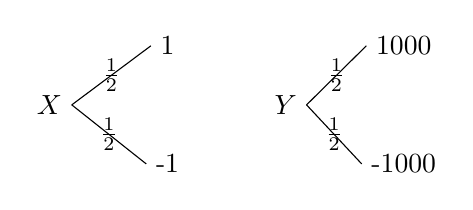
\begin{tikzpicture}[grow'=right]
	\begin{scope}
	\node{$X$}
	child{
		node{1}
		edge from parent node {\half}	
	}
	child{
		node{-1}
		edge from parent node {\half}	
	};
	\end{scope}
	
	\begin{scope}[xshift=3cm]
	\node{$Y$}
	child{
		node{1000}
		edge from parent node {\half}	
	}
	child{
		node{-1000}
		edge from parent node {\half}	
	};
	\end{scope}
	
	
	\end{tikzpicture}
\end{center}

The expected value of both games are 0. But $Y$ seems way more risky than $X$ and the reason is the variance.

The variance of $X$ is given by
\[
	\Var[X] = \half \times (1-0)^2 + \half \times (-1-0)^2 = 1
\]

The variance of $Y$ is given by
\[
	\Var[Y] = \half \times (1000-0)^2 + \half \times (-1000-0)^2 = 1000^2
\]


\example Let us consider rolling one fair dice and let
\[
	R(\omega) = \text{ The face of the dice.}
\]
Let us find the variance of value on the face of the dice.

First, we need to find the expected value $\E[R]$. This is simply 3.5 as we found in one of previous example.

Then, we need to find
\begin{align*}
	\E\left[(R - \E[R])^2\right] =& \E\left[(R - 3.5)^2\right]\\
	=& (1-3.5)^2 \Pr(R=1)  \\
	&+(2-3.5)^2 \Pr(R=2)  \\
	&+\ldots + (6-3.5)^2 \Pr(R=6)\\
	=& \frac{1}{6} (2.5^2 + 1.5^2 + \ldots + 2.5^2)\\
	= & \frac{35}{12}
\end{align*}

Sometimes it is more useful to report the standard deviation instead of variance since it has the same unit has the random variable itself. So it gives you the sense of width of distribution.

\definition The standard deviation of a random variable $R$ is given by
\[
	\sigma_R = \sqrt{\Var[R]}.
\]
which is just the square root of the variance ($\sigma$ reads sigma).

Variance and standard deviation contains exactly the same information. Variance is much easier to work with since it is an expected value. The standard deviation give you more intuitive picture about the distribution of the random variable.

%INSERT PICTURE HERE....

\section*{Alternative Method}

There is another way to calculate the variance.

\theorem Given a random variable $R$ the variance can also be found by
\[
	\Var[R] = \E[R^2] - \E[R]^2
\]

\proof We start with the definition of variance.
\begin{align*}
	\Var[R] =& \E[(R - \E[R])^2]\\
	=& \E\left[ R^2 - 2 R \E[R] + \E[R]^2\right]\\
	\expl{=}{Linearity}& \E[R^2] - \E[2 R \E[R] ] + \E[\E[R]^2]\\
	\expl{=}{$2 \E[R]$ is constant}& \E[R^2] - 2 \E[R]^2 + \E[\E[R]^2]\\
	\expl{=}{$\E[R]^2$  is a constant}& \E[R^2] - 2 \E[R]^2 + \E[R]^2\\
	=& E[R^2] - E[R]^2
\end{align*}
\qedd


\example Let us consider the the game where you can win $2$ Baht with probability $\frac{2}{3}$ or lose $1$ Baht with probability $\frac{1}{3}$. Let us find the variance.

Method 1: let us use the first definition. We know that
\[
\E[R] = 2 \times \frac{2}{3} - 1 \times \frac{1}{3} = +1 
\]
So the variance is
\begin{align*}
	\Var[R] = (2-1)^2 \cdot \frac{2}{3} + (-1-1)^2 \cdot \frac{1}{3} = 2
\end{align*}

Method 2: Let us use what we just prove right here. Let us find
\[
	\E[R^2] = 2^2 \cdot \frac{2}{3} + (-1)^2 \cdot \frac{1}{3} = 3.
\]
So, the variance is given by
\[
	\Var[R] = \E[R^2] - \E[R]^2 = 3-1 = 2,
\]
which is the same answer as method 1.

\example Variance of indicator random variable. Let us consier a random variable $B$ defined by
\begin{center}
	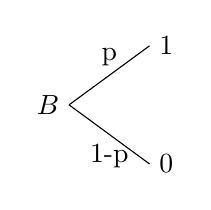
\begin{tikzpicture}[grow'=right]
		\node{$B$}
		child{
			node{1}
			edge from parent node[above] {p}	
		}
		child{
			node{0}
			edge from parent node[below] {1-p}	
		};
	\end{tikzpicture}
\end{center}

The variance of $B$ is given by
\[
	\Var[B] = \E[B^2] - \E[B]^2 = p-p^2 = p(1-p)
\]

\example Variance of a uniform random variable. Let us consider the variance of the face of a fair dice roll($D$).

We need to find
\[
	\E[D^2] = \frac{1}{6} (1^2 + 2^2 +\ldots 6^2) = \frac{91}{6}
\]
and the mean is
\[
	\E[D] = \frac{7}{2}
\]

So, the variance is given by
\[
	\Var[D] = \E[D^2] - \E[D]^2 = \frac{35}{12}
\]

\section*{Variance Property}

\subsection*{Constant Additions}

Let us consider the variance of $R$ added by a constant. If you picture the variance as a measure of the width of the distribution then shifting the graph by adding a constant does not do anything to the width at all. That means $\Var[R+c] = \Var[R]$. But, we are going to prove it properly.

\theorem Let $R$ be a random variable and $c$ be a real number then
\[
	\Var[R] = \Var[R+c]
\]

\proof Let us consider $\Var[R+c]$.
\begin{align*}
	\Var[R+c] =& \E\left[(R+c - \E[R+c])^2\right]\\
	\expl{=}{Linearity}& \E\left[\left(R+\cancel{c} - (\E[R] + \cancel{c}) \right)^2\right]\\
	=& \E[(R - \E[R])^2]\\
	=& \Var[R]
\end{align*}
\qedd

\subsection*{Constant Multiplications}

This is the part where most people guess the wrong answer. A lot of people would have thought that
\[
	\xcancel{\Var[aR] = a \Var[R]}.
\]
But this is completely wrong since if $a$ has a unit then the left and the right hand side doesn't even have the same unit. Let us find the correct way to do it.

\theorem Let $R$ be a random variable and $a$ be a real number then
\[
	\Var[aR] = a^2\Var[R]
\].
Do not forget the square on $a$.

\proof Let us consider $\Var[aR]$.
\begin{align*}
	\Var[aR] =& \E\left[ (aR - \E[aR])^2 \right]\\
	\expl{=}{Linearity}& \E\left[ (aR - a\E[R])^2 \right]\\
	=& \E\left[ a^2(R - \E[R])^2 \right]\\
	\expl{=}{Linearity}& a^2 \E\left[ (R - \E[R])^2 \right]\\
	=& a^2 \Var[R]
\end{align*}

\subsection*{Variance of Sum}

\theorem Let us consider two random variable $R_1$ and $R_2$ not necessarily independent. Then,
\[
	\Var[R_1 + R_2 ] = \Var[R_1] + \Var[R_2] + 2\Cov[R_1,R_2]
\]
where
\[
	\Cov[R_1,R_2] = \E[R_1 R_2] - \E[R_1]\E[R_2]
\]
\proof By definition,
\begin{align*}
	\Var[R_1 + R_2] =& \E\left[(R_1 + R_2)^2 \right] -  \E\left[R_1 + R_2 \right]^2\\
	\expl{=}{Linearity}& \E\left[(R_1 + R_2)^2 \right] -  (\E[R_1] + \E[R_2])^2\\
	=& \E\left[(R_1 + R_2)^2 \right] \\
	&-\left(\E[R_1]^2 + 2\E[R_1]E[R_2] +\E[R_2]^2 \right)\\
	=& \E\left[R_1^2 + 2 R_1 R_2 + R_2^2 \right] \\
	&-\left(\E[R_1]^2 + 2\E[R_1]E[R_2] +\E[R_2]^2 \right)\\
	=& \E[R_1^2] + 2\E[R_1 R_2] + \E[R_2^2] \\
	&-\left(\E[R_1]^2 + 2\E[R_1]E[R_2] +\E[R_2]^2 \right)\\
	=& \E[R_1^2] - \E[R_1]^2 + \E[R_2^2] - \E[R_2]^2\\
	&+ 2\E[R_1 R_2] - 2\E[R_1]\E[R_2]\\
	=& \Var[R_1] + \Var[R_2] \\
	& + 2\E[R_1 R_2] - 2\E[R_1]\E[R_2]\\
	=& \Var[R_1] + \Var[R_2] + 2\Cov[R_1,R_2]
\end{align*}
\qedd

You would have expected to just add up the variance but there is a pesky covariance term at the end. This makes sense since if the two random variabls gives the same value every time then we expect the variance to be 4 times the original one not just two.

But, if the two random variable are independent then we have a very nice formula since the covariance becomes zero. Let us prove this fact.

\theorem If $R_1$ and $R_2$ are indpendent then
\[
	\Cov(R_1, R_2) = 0.
\]
It should be noted that the converse is however not true.

\proof By definition
\[
	\Cov[R_1, R_2] =  \E[R_1 R_2] - \E[R_1]\E[R_2]
\]
Since $R_1$ and $R_2$ are independent the first time is simply
\[
	\Cov[R_1, R_2] =  \E[R_1]\E[R_2] - \E[R_1]\E[R_2] = 0
\]
\qedd

The converse is however not true. Let us take $A$ and $B$  to be independent random variable which takes the value -1 or +1 with probability of 0.5 each. Then, we can consider $X=A+B$ and $Y=A-B$. You can find that the covariance is 0 but the $X$ and $Y$ are not independent. Do it as an exercise.

\collorary If $R_1$ and $R_2$ are \emph{independent} then we have a nice formula
\[
	\Var[R_1+R_2] = \Var[R_1] + \Var[R_2]
\]
\proof This is because the covariance is 0.

\example This gives us a very nice formula for finding the variance of a binomial distribution. All we need to do is write the random variable as a sum of independent indicator random variable. Each of the indicator random variable has probability $p$ of being 1 and $1-p$ of begin 0.

Since
\[
	R = R_1 + R_2 + \ldots R_n,
\]
the variance is just
\begin{align*}
	\Var[R] =& \Var[R_1] + \Var[R_2] + \ldots \Var[R_n]\\
	=& p(1-p) + p(1-p) + \ldots p(1-p)\\
	=& np(1-p)
\end{align*}

\subsection*{Covariance and Correlation}

\definition Alternate definiton of covariance. Let $X$ and $Y$ be two random variable. The covariance of $X$ and $Y$ is given by
\[
	\Cov[X,Y] = \E[ (X-\E[X])(Y-\E[Y])]
\]

Showing that the two definiton are equivalent is just a matter of using linearity of expectation which is very similar to how we got the formula for how to calculate the variance.

This relation makes it easy to see that
\[
	\Cov[X,X] = \Var[X]
\]

You may ask what exactly does covariance represent. It quantify whether if $X$ is above mean does that tell us something about whether $Y$ is also above the mean.

For example, let us consider the case where everytime $X$ is above the mean $Y$ is also above the mean and every time $X$ is below the mean then $Y$ is below the mean. This mean that every terms in the expected value are positive; whenever the first time is positive the second term is positive and whenever the first term is negative the second term is negative. This means that the product is always positive.

In the opposite case where whenver $X$ is above the mean $Y$ is below the mean and vice versa. Every term in the sum is negative. So, the covariance will be a very negative value.

\subsection*{Correlation Coefficient}

The covariance is quite inconvenient to interpret since it depends on the scale of the random variable. For example, the covariance of $aX$ and $Y$ is given by
\[
	\Cov[aX,bY] = ab \Cov[X,Y]
\]
the proof is left for the reader as an exercise. We can fix this problem by defining a correlation coefficient.

\definition Correlation Coefficient. The correlation coefficient of two random variable $X$ and $Y$ is given by
\[
	\rho_{X,Y} = \frac{\Cov(X,Y)}{\sigma_X \sigma_Y}
\]

First thing you notice is that the scale dependent is gone. In fact, it is much better than that.

\theorem Let $X$ and $Y$ be two random variables. Then the correlation is bounded by
\[
	-1 \le \rho_{X,Y} \le 1
\]

\proof This is actually related to Cauchy-Schwarz inequality. Let us prove it here. The proof is a quite clever so look closely. Quite a useful technique though.

Let us consider $\E[(U + tV)^2]$ where $U = X-\E(X)$ and $V=Y-\E(Y)$, since every term in the expected value is postive. The expected value is positive(or zero)
\[
	\E[(U + tV)^2] \ge 0
\]

Let us expand it
\[
	\E[U^2 + 2t UV + t^2V^2] \ge 0
\]

The linearity of expectation tells us
\[
	\E[U^2] + 2 t \E[UV] + t^2\E[V^2] \ge 0
\]

But, $\E[U^2]=\sigma_X^2$ ,$\E[V^2] =\sigma_Y^2$ and $\E[UV] = \Cov(X,Y)$. You can verify this as an exercise.

This means that we have
\[
	t^2 \sigma_Y^2 + 2 t \Cov[X,Y] + \sigma_X^2 \ge 0
\]

The minimum of the left hand side happens at (take derivative set it to zero)
\[
	t = -\frac{\Cov[X,Y]}{\sigma_Y^2}
\]

Plug this back in give
\begin{align*}
	\text{Min LHS} =& -\frac{\Cov[X,Y]^2}{\sigma_Y^2} + -2\frac{\Cov[X,Y]^2}{\sigma_Y^2} + \sigma_X^2\\
	=& -\frac{\Cov[X,Y]^2}{\sigma_Y^2} + \sigma_X^2
\end{align*}

This minimum still has to be greater than 0. This means
\begin{align*}
	-\frac{\Cov[X,Y]^2}{\sigma_Y^2} + \sigma_X^2 \ge& 0\\
	\sigma_x^2 \ge& \frac{\Cov[X,Y]^2}{\sigma_Y^2}\\
	1 \ge& \left( \frac{\Cov[X,Y]}{\sigma_X \sigma_Y} \right)^2\\
	1 \ge& \rho_{X,Y}^2
\end{align*}

Therefore,
\[
-1 \le \rho_{X,Y} \le 1
\]
\qedd

This limits make the correlation coefficient easier to interpret than the covariance. Since the number is between $-1$ and $1$. One and minus one means fully correlated/anti-correlated one random variable is just a linear combination of another random variable.

So, we can rewrite the fomula for combining the variance as
\[
	\Var[X+Y] = \sigma_{X+Y}^2  = \sigma_X^2 + \sigma_Y^2 + 2 \sigma_X \sigma_Y \rho_{X,Y}
\]
You will be using this formula to find how to minimize risk in stock picking in the homework.
\end{multicols}




\end{document}
